\documentclass{DenebClass}

\title{Deneb Kaitos - La Marque des Ergios}
\author{Lionel "Armaklan" ZUBER}
\begin{document}
\maketitle
\clearpage

\chapter{L'univers}

\begin{multicols}{2}

\begin{center}
	\includegraphics[width=113pt]{../Img/velios}
\end{center}

\section{La situation actuelle}

De nouveau, la guerre a éclaté... N'apprendrons nous jamais de nos erreurs ? La longue période d'anarchie qui a suivi les départs des Ergios ne nous as visiblement pas suffit. L'alliance Kaitienne, dans sa soif de pouvoir, n'a pas tenu compte de l'avis de la Fédération. Celle-ci a exploser en morceau. Les anciens conflits rejaillissent comme si la paix n'avait jamais existé. 

L'alliance Kaitienne a ouvert le feu mais tous guettaient la reprise des hostilités ! Il n'a pas fallu longtemps pour que les grands vaisseaux de métal de l'alliance Terrienne affrontent les nombreux Teldrims et leurs troupes galvaniser par la prêtrise du Protectorat. 

Les Snagirs, jusqu'alors pacifique et diplomate ont soudain changé de méthode ! Le Consortium, la plus grande corporation Snagir vient de faire un coup d'état et de prendre les rennes de leurs gouvernements, forçant la lourde mécanique administrative Snagir à réagir et à passer à l'offensive. 

Les Corporations, devenus multi-stellaire durant la période de paix, se sont lassées de la politique des gouvernements actuels. A la stupeur de tous, les principales corporations ont fondées le Bureau Corporatiste, un gouvernement sous leurs directions directs. Le Bureau Corporatiste s'est alors principalement opposé à l'Alliance Kaitienne. Ils ont déjà prit à l'alliance plusieurs systèmes, entrainant le déclin d'une puissance jusqu'alors dominante. 

Et comme si tous cela ne suffisait pas, une nouvelle race est apparus, les "Eskador". Ces créatures sortis de nulle part ont ravagé une partie de Kaitos, l'ancienne capitale. Ils ont alors été repoussée uniquement au prix de très lourde perte. Qui sont ces nouveaux venus ? Que veulent ils ? Pour l'instant personne n'a pu rentrer en contact avec eux, leurs rares apparitions sont toujours des interventions militaires. 

L'attaque des Eskadors a été terrible pour les mondes connus ! Seul l'intervention de l'empire Vélïos, qui avait cessé tout contact depuis des siècles, a permis de repousser cet étrange envahisseur. Pourquoi les Vélïos ont-il choisit ce moment pour revenir ? Que prépare t'il ?

Quels va être l'avenir des mondes connus ? Une nouvelle Fédération ? Un gouvernement unifié par le Bureau Corporatiste ? Survivront nous au moins au Eskador ? A moins que l'Aube Pourpre, cette secte terroriste n'est raison, et que les Ergios décident de revenir..

\begin{center}
	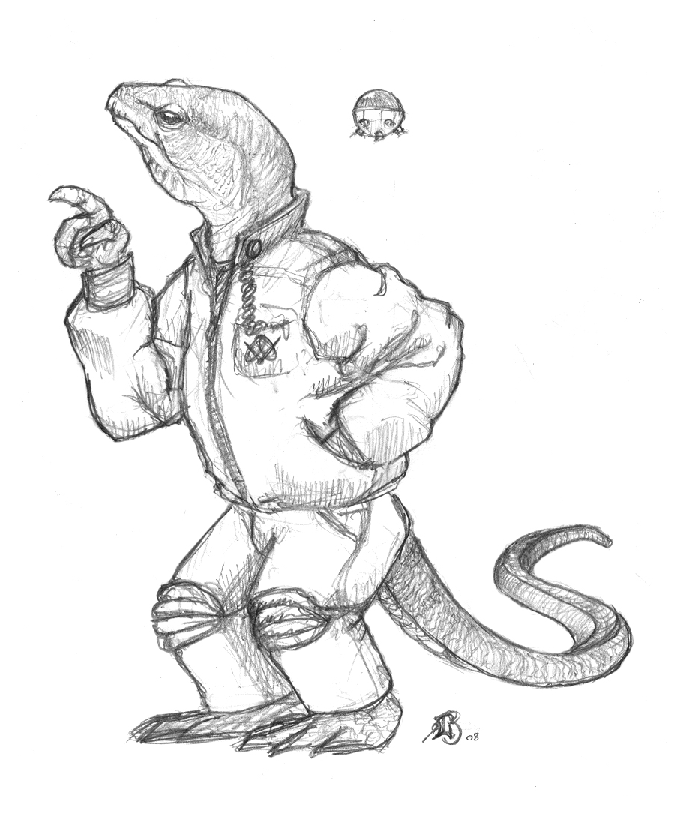
\includegraphics[width=140pt]{../Img/snagir}
\end{center}

\begin{center}
	\includegraphics[width=170pt]{../image/vaisseau5}
\end{center}

\section{Les Peuples}

Deneb Kaitos propose d'interprété des personnages venants de l'un des 6 peuples suivants :

\begin{itemize}
\item Les Humains, descendant direct des Terriens. Les Terriens ont la réputation d'être des comédiens et manipulateur né. 
\item Les Centauriens, de lointains cousins qui ont muter en une nouvelle espèce à cause de leurs expositions aux radiations émis par Alpha du Centaure. Les Centauriens sont tous liés entre eux par un lien télépathique.
\item Les Teldrims, des sortes d'homme-félin qui se laisse gouverner par leurs instincts de prédateurs. Les Teldrims sont êxtremement réligieux. Réparti en 6 espèce, l'une d'entre elle est considéré comme une race esclave.
\item Les Snagirs, des hommes lézards pour qui la technologie n'a aucun secret. Seule le savoir et la réalisation technologique à une valeur chez eux.
\item Les Vélïos, un peuple de guerrier à la musculature développés et au sens de l'honneur inscrit dans le marbre. Les Vélïos sont dotés dans le dos d'une paire de lame dorsale qui les rends extrêmements dangereux. 
\item Les Nomades, venant de toutes les races, et ayant décidé d'abandonner totalement la terre ferme au profit de la vie dans l'espace : Vaisseau, Station Spatiale, Astéroïde, ... Avec le temps les nomades ont acquis une culture qui leurs est propre et une très grande indépendance vis à vis des "planétaires".
\end{itemize}

\section{La Marque des Ergios}

Quelques pouvoir psy existe dans les mondes connus : le lien télépathique des centauriens, le capacité des prêtres Teldrims à modeler leurs bois sacrés par la pensée, ... Ces pouvoirs sont toutefois faible, difficile à mettre en oeuvre, et extrêmement fatiguant pour ceux qui en sont dotés.

Mais depuis peu nous observons un nouveau phénomène. Certains personnages sont dotés de ce que l'on appelle "La Marque des Ergios". Cette marque, invisible en temps normal, apparait lorsque son possesseurs utilise des pouvoirs psychique. Les personnages portant cette marque ont accès à des pouvoirs jusqu'alors inconnus, et ceux avec une déconcertante éfficacité.

Quel est cette marque ? Quel est son rôle ? Qui sont les "marquées ?" Autant de questions qui sont sans réponses. Même les marqués n'en savent rien. 


\begin{center}
	\includegraphics[width=180pt]{../Img/teldrim_psy}
\end{center}


\begin{center}
	\includegraphics[width=160pt]{../image/vaisseau1}
\end{center}

\section{Que jouer ?}

Les personnages joueurs portent tous la Marque des Ergios. Cette marque est extrêmement rare. Le pouvoir psychique des possesseurs de cette marque les rendres extrêmement précieux. En ces temps troubles, les porteurs de Marques pourront surement décidés le destin du monde connus.

Deneb Kaitos a pour objectif de faire vivre aux personnages des aventures plus grandes que natures. Les personnages sont exceptionnels et extrêmement puissant, ils vont donc très vite se retrouver aux centres des intrigues. Leurs actes, leurs paroles influencera le destin des mondes connus...

\end{multicols}

\chapter{Le système de jeu}

\begin{multicols}{2}

Deneb Kaitos utilise le système Fusina, un système de jeu en creative commons.

\section{Objectif du système}

Fusina est un système de jeu de rôle qui se veut "Simple, fun, et narratif". A ces trois termes nous tenons également à rajouter "Cinématique". Fusina se veut donc facile à prendre en main et à adapter à un nouvel univers. Le système à pour objectif de placer les personnages aux centres de l'attention et de promouvoir le jeu "d'histoire" en lieu et place du jeu dit "stratégique". La force de Fusina est une gestion unifié de toutes les situations, du simple duel à l'épée jusqu'au combat spatiale épique engageant des forces gigantesques, tous sera geré de manière identique. 

Vous ne voulez pas vous prendre la tête ? Vous voulez pouvoir jouer rapidement ? Vous aimez avant tous l'histoire ? Vous aimez le panache et les grandes descriptions ? Fusina est fait pour vous ! Vous aimez les systèmes complexes où ils faut réflechir longuement à quels est la meilleur option, alors passez votre chemin, Fusina ne vous conviendra pas.

\section{La base du système}

Le système s'appuie sur différents types d'élements assez classique :

\begin{itemize}
\item Les caractéristiques
\item Les compétences
\item L'équipement
\item Les traits
\item Les faiblesse, handicaps, et blessure
\end{itemize}

\begin{center}
	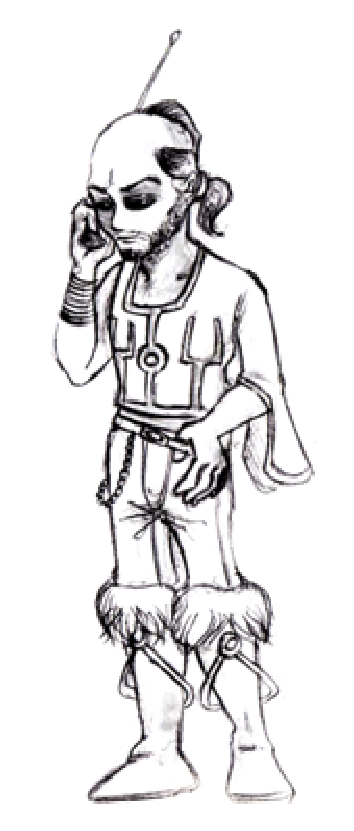
\includegraphics[width=90pt]{../Img/centaurien}
\end{center}


Les caractéristiques, compétences et équipements sont représentées à l'aide d'une valeur chiffrées indiquant un type de dé allant de D4 à D12. Lors d'une action, le personnage va lancer un dé pour la caractéristique (au minimum), un dé pour la compétence utilisée le cas échéant, et un ou plusieurs dé pour l'équipement. Il devra ensuite choisir un résultat parmis ceux obtenus. Le résultat sera ensuite opposé au résultat adverse (opposition) ou à un seuil de difficulté.

Les traits sont quelques mots, courtes phrases, ou expression reflétants les aspects positifs du personnage. Les traits ne sont pas chiffrées mais pourra apporter des bonus sous différentes formes (+2, relance, ou explosion selon les variantes choisies pour le système).

Les faiblesses sont des traits indiquant le coté négatif du personnage. Les handicaps représentent tous ce qui peut géner le personnage dans l'accomplissement d'une action. Ces handicaps arrivent en général suite à des oppositions. Les blessures sont des handicaps dues à une opposition longue et souvent physique. Ces trois élements intéragissent de manière strictement identique lors des actions. Ils ont pour effet de limiter les résultats que le personnage peut choisir, et donc à précipiter l'échec.

Particularité de Fusina, la description d'une action se fait toujours une fois les jets effectués. C'est au joueur qu'incombe la description. Le MJ se contente d'indiquer le type de réussite (de justesse, large, ...) et de guider les joueurs dans leurs descriptions.

\section{Panache et Stress}

Le Panache et le Stress sont deux pools de points disponible pour les joueurs. Le Stress est toujours accessible aux joueurs, quand ils le dépensent le stress est alors disponible pour le maitre du jeu. Le Panache à un accès plus limité : c'est au mj de la distribuer aux joueurs pour bonne idée, bonne action, bon roleplay, ...

Le Panache et le Stress se dépensent de manière identique. Ils permettent d'obtenir des bonus lors des actions (utilisation d'un trait, ignorer une faiblesse, +1, ...) et sont, en général, nécessaire à l'utilisation de pouvoir Psy/Magique.

\end{multicols}


\begin{center}
	\includegraphics[width=350pt]{../Img/aube_pourpre.png}
\end{center}

% LaTeX2e code generated by txt2tags 2.6 (http://txt2tags.org)
% cmdline: txt2tags -t tex deneb.t2t
\end{document}
